
% \pagenumbering{arabic}
% \setcounter{page}{1}


\chapter{Background} \label{sec:background}


In this chapter, we explain the basic concepts required for comprehending this dissertation.



\section{Blockchain}
Public blockchains are the most promising underlying technology for many applications. They are aiming to be decentralized, transparent, and immutable. However, they are also slow, expensive, and have limited functionality. They can and will replace many intermediary entities we know of today. However as we will dive deeper in this subject, blockchain, as a technology is in its infancy. The public aspect of these blockchains changes many assumptions developers and system designers have about the data flow within their applications. 

Blockchain works by having a decentralized network of nodes that are incentivized to maintain the network. The nodes are incentivized by receiving rewards in the form of cryptocurrency. The nodes are also responsible for verifying the transactions and adding them to the blockchain. The blockchain is a chain of blocks, each block containing a list of transactions. The order of the transactions in each block is important as it indicates the order of events in the blockchain.


\begin{figure}[h]
    \centering
    {\caption{The building blocks of blockchain technology~\cite{gaggioli2019middleman}}}
    {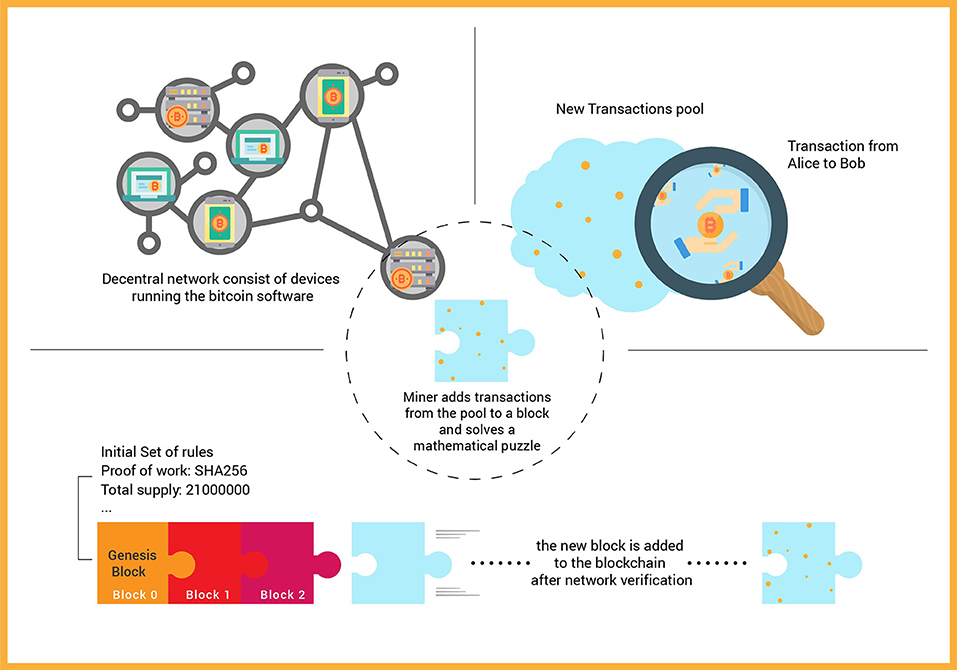
\includegraphics[width=0.8\textwidth]{figures/blockchain-buildingblocks.jpg}}
    \end{figure}
    %https://www.lucidchart.com/invitations/accept/f8ca2662-5269-425d-9deb-deb14af2aac7


This technology has the potential of many interesting applications, from digital cash (\eg Bitcoin~\cite{nakamoto2008bitcoin}), prediction markets~\cite{clark2014decentralizing}, and decentral governance~\cite{aragonwebsite}. Bitcoin, started in 2009, was the first application of blockchain technology and since then the concept of decentral ledger has grown to many other applications that just a ledger holding transaction data. 


\section{Ethereum}

Ethereum~\cite{wood2014ethereum} is a prominent public blockchain that has attracted the largest developer headcount compared to other blockchains. It is an extension of its predecessor, Bitcoin~\cite{nakamoto2008bitcoin}, but with significant enhancements, notably the addition of \textit{smart contracts}. These smart contracts are applications residing on the blockchain that can immutably execute their verified code. Ethereum operates on a Turing-complete virtual machine, the \texttt{Ethereum Virtual Machine (EVM)}, allowing programs to live and be executed on the blockchain. This differs from Bitcoin's UTXO\footnote{Unspend Transaction Output} model, which primarily supports value transfers and has a scripting language for extending transaction functionality to a limited extent. In contrast, Ethereum's Turing-complete language opens up limitless possibilities.  All transactions and executions on Ethereum are verified by a decentralized network of nodes. The nodes are incentivized to verify transactions and execute smart contracts by receiving rewards in the form of Ether, the native cryptocurrency of Ethereum. 

Ethereum blockchain started in 2015 using the similar consensus mechanism as Bitcoin, called Proof of Work (PoW), also known as mining. However, in 2020, Ethereum started the transition to Proof of Stake (PoS) consensus mechanism. The main difference between PoW and PoS is that in PoW, the nodes are incentivized to solve a computationally hard puzzle to be able to add a block to the blockchain. However, in PoS, the nodes are incentivized to stake their Ether to be able to add a block to the blockchain. The PoS mechanism is more energy efficient and more scalable than PoW. Ethereum fully switched to PoS in September 2022 in an event called the \textit{Merge}, and reduced its energy consumption by 99.5\%~\cite{themerge}. In this dissertation, we do not directly focus on the consensus mechanisms, however, we will discuss the implications of the consensus mechanism on the blockchain security in chapter ~\ref{sec:frontrunning}. 


\subsection{Smart Contracts}
Smart contracts, a fundamental component of blockchain technology, particularly in the Ethereum ecosystem, represent a paradigm shift in how contractual agreements are executed and enforced. These contracts are essentially codebases that reside on the blockchain, acting as autonomous agents that carry out predefined functions when a user invokes the contract and certain conditions are met. 

At their core, Ethereum smart contracts are collections of code and data (state) residing at a specific address on the Ethereum blockchain. Developed primarily in Solidity, a high-level language specifically designed for Ethereum, these contracts encapsulate a set of rules and automatically enforce them through the code. Solidity, with its syntax similar to JavaScript and C++, enables developers to write applications that implement self-enforcing business logic encapsulated within smart contracts, thereby removing the need for intermediaries.

Smart contracts are compiled into bytecode and deployed on the Ethereum blockchain. Once deployed, they become immutable – their code cannot be altered, ensuring the integrity of the contract. Execution of a smart contract is triggered by transactions. These transactions are sent by external Ethereum accounts, containing the necessary information to invoke specific functions within the contract. Every operation in a smart contract requires a certain amount of \textit{gas}, a unit that measures the computational effort required to execute operations. Users initiating transactions must supply enough Ether, Ethereum's native cryptocurrency, to cover the gas costs, which are determined by the complexity of the operations and the current network demand. This mechanism prevents inefficient or malicious contracts from wasting network resources. Smart contracts maintain an internal state stored on the blockchain. This state can include variables, balances, and other contract-specific data. When a contract's function is executed, it can alter its state (e.g., updating balances, changing ownership records) and can also interact with other contracts, thereby enabling complex decentralized applications (DApps).

While Ethereum smart contracts offer a wide range of functionalities, they are not without limitations. Their capabilities extend from creating tokenized assets and managing digital identities to executing decentralized finance (DeFi) transactions and running complex DApps. Use cases like decentralized gambling platforms, voting systems, and automated payroll services exemplify their versatility. However, the "unstoppable" nature of these contracts also poses challenges, particularly in terms of security and scalability. The code's immutability means that any flaws or vulnerabilities in the contract cannot be easily rectified post-deployment, emphasizing the need for rigorous testing and auditing pre-deployment. Security in smart contracts is paramount, as vulnerabilities can lead to significant financial losses. Common issues include reentrancy attacks, where a malicious contract can repeatedly call a function in the original contract, and problems arising from visibility and access control, where private data or functions can be unintentionally exposed. 

As noted earlier, everything on a blockchain is compromised of transactions and blocks. The order of the transactions in each block indicates the order of events and smart contract executions in the Ethereum blockchain. Given that miners, and recently entities named \textit{block builders}, are in control of the order, it is possible for these entities to reorder the transaction in a block, or even not include a transaction in a block for higher financial gain from the new order. This is the basics of blockchain front-running that we discuss in the next chapters. 


\subsection{P2P Network}
The Ethereum network, envisioned as a global, decentralized computer, operates on a peer-to-peer (P2P) basis, a key feature that distinguishes it from traditional centralized systems. This P2P architecture is foundational to Ethereum's functionality, enabling a trustless and permissionless environment where anyone can participate in the network. In the core of the design principles of Ethereum's P2P network, there are three main concepts: decentralization, trustless interactions, and permissionless nature. These concepts are the foundation of the Ethereum network and are the main reasons for the success of Ethereum.

\paragraph{Decentralization and Accessibility:} Ethereum's network is designed to be fully decentralized, eliminating any central point of control or failure. This decentralization ensures that the network remains resilient against attacks and censorship. It is worthy to note that these are the ideal properties and the current state of the network does not have full resiliency against these attacks. The accessibility of the network allows anyone to run a full node, contributing to the network's health and security.

\paragraph{Trustless Interactions:} In Ethereum's P2P network, nodes interact without needing to trust each other. Trustlessness is achieved through cryptographic verification methods and consensus algorithms, ensuring that all transactions and blocks adhere to the network's rules without requiring mutual trust among participants.

\paragraph{Permissionless Nature:} The network's permissionless design means that anyone can join and leave the network at will, participate in mining activities, and contribute to the network's consensus process. This open-access principle is fundamental to Ethereum's ethos of inclusivity and decentralization.

As Ethereum has grown in popularity, the network has faced scalability issues, leading to congestion and high transaction fees. Solutions like sharding, which splits the network into smaller partitions, and layer-2 scaling solutions like rollups, are being developed to address these challenges. 



\subsection{Nodes}

The Ethereum network comprises various types of nodes, including archival nodes, full nodes, and light nodes. Archival nodes store everything including all the state transitions which are not required to verify the latest state of the blockchain. Full nodes store the entire blockchain, validate transactions and blocks, and enforce consensus rules. Light nodes, designed for less resource-intensive operations, download only the header chain and request necessary data from full nodes. Nodes communicate using a P2P protocol, exchanging information such as transactions, blocks, and node data. This communication is facilitated by protocols like the Ethereum Wire Protocol~\cite{ethereumwireprotocol}, which manages the synchronization of node data and the propagation of new blocks and transactions.


\subsubsection{mempool}
When an Ethereum transaction is initiated, it first undergoes validation by a participating node in the network. This validation process includes verifying the transaction's signature and ensuring the sender has sufficient funds. Post-validation, the node disseminates the transaction across the network. Prior to its inclusion in a blockchain block, this transaction resides in what is known as the "mempool" (or memory pool) of each node. The mempool functions as a holding area for all pending transactions. Due to the asynchronous nature of transaction reception, each node may have a differently ordered mempool, as transactions are received and stored in the order they arrive.

The mempool in Ethereum nodes plays a crucial role in the transaction processing mechanism. It acts as a sort of waiting room for transactions before they are confirmed and added to a block. Each node in the Ethereum network maintains its own mempool, and there is no universal consensus on the order of transactions within these individual mempools. This is primarily because transactions reach different nodes at different times, leading to varying sequences.

Block builders (previously miners), who are responsible for creating new blocks, typically select transactions from their mempool. They often prioritize transactions with higher gas fees, as this maximizes their profit from block rewards and transaction fees. The decentralized and varied nature of mempools allows block builders to reorder transactions. This can be exploited for financial gain, a practice known as "transaction reordering" or "front running." They may choose transactions based on the transaction fees offered, leading to scenarios where transactions with higher fees are processed faster, while others with lower fees might experience delays.
The mempool is a dynamic component of the Ethereum network, constantly changing with the arrival of new transactions and the creation of new blocks. It reflects the fluid nature of the network’s transactional throughput and is a critical element in understanding Ethereum's operational mechanics. As the network evolves, managing the mempool efficiently remains a key challenge, particularly in addressing issues like network congestion, transaction prioritization, and the ethical implications of transaction reordering.